\documentclass[]{BasiliskReportMemo}
\usepackage{AVS}
\usepackage{algorithmic}
\usepackage[boxed]{algorithm}


\newcommand{\submiterInstitute}{Autonomous Vehicle Simulation (AVS) Laboratory}

\newcommand{\ModuleName}{ThrusterForces}
\newcommand{\subject}{Algorithms to Map Desired Torque Vector onto a set of Thrusters }
\newcommand{\status}{Initial Draft}
\newcommand{\preparer}{H. Schaub}
\newcommand{\summary}{Include a short summary of what this system engineering report is about.  Should be 300 words or less.     }


\begin{document}


\makeCover


%
%	enter the revision documentation here
%	to add more lines, copy the table entry and the \hline, and paste after the current entry.
%
\pagestyle{empty}
{\renewcommand{\arraystretch}{1.1}
\noindent
\begin{longtable}{|p{0.5in}|p{4.5in}|p{1.14in}|}
\hline
{\bfseries Rev}: & {\bfseries Change Description} & {\bfseries By} \\
\hline
Draft & XXXXXX & X. XXXX \\
\hline

\end{longtable}
}

\newpage
\setcounter{page}{1}
\pagestyle{fancy}

\tableofcontents
~\\ \hrule ~\\

\begin{figure}[htb]
	\centerline{
	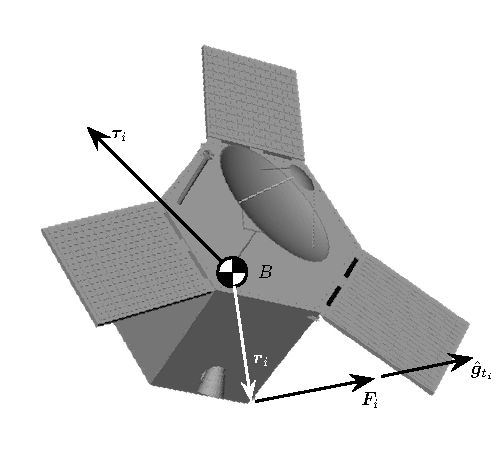
\includegraphics[]{Figures/thrusterNotation}
	}
	\caption{Illustration of the Spacecraft Thruster Notation}
	\label{fig:thruster}
\end{figure}

\section{Introduction}
This technical note describes a general algorithm that maps a desired ADCS external control torque $\bm L_{r}$ onto force commands for a cluster of thrusters.  The body fixed frame is given by $\frameDefinition{B}$.  The $j^{\text{th}}$ component of $\bm L_{r}$ is given by
\begin{equation}
	L_{r,j} = \bm L_{r} \cdot \hat{\bm b}_{j}
\end{equation}�

The $i^{\text{th}}$ thruster location relative to the spacecraft point $B$ is given by $\bm r_{i}$ as illustrated in Figure~\ref{fig:thruster}.  The unit direction vector of the thruster force is $\hat{\bm g}_{t_{i}}$, while the thruster force is given by
\begin{equation}
	\label{eq:th:1}
	\bm F_{i} = F_{i} \hat{\bm g}_{t_{i}}
\end{equation}
The toque vector produced by each thruster about the body fixed point $B$ is thus
\begin{equation}
	\bm \tau_{i} =\bm r_{i} \times F_{i}  \hat{\bm g}_{t_{i}}
\end{equation}
The total torque onto the spacecraft about the $j^{\text{th}}$ body fixed axis, due to a cluster of $N$ thrusters, is
\begin{equation}
	\tau_{j} = \sum_{i=1}^{N} \bm \tau_{i} \cdot \hat{\bm b}_{j}
	= \sum_{i=1}^{N}  (\bm r_{i} \times \hat{\bm g}_{t_{i}})\cdot \hat{\bm b}_{j} F_{i} = \sum_{i=1}^{N}  d_{i} F_{i}
\end{equation}
where 
\begin{equation}
	d_{i} =   (\bm r_{i} \times \hat{\bm g}_{t_{i}})\cdot \hat{\bm b}_{j}
\end{equation}
In matrix form, the net spacecraft torque about the $j^{\text{th}}$ axis is written compactly as
\begin{equation}
	 \tau_{j} = \begin{bmatrix}
		 d_{1} \cdots  d_{N}
	\end{bmatrix} \begin{bmatrix}
		F_{1} \\
		\vdots \\
		F_{N}
	\end{bmatrix} = [D] \bm F
\end{equation}
where $[D]$ is a $1\times N$ matrix that maps the thruster forces $F_{i}$ to the spacecraft torque $\tau$. 

The thruster control goal is to find a set of thruster forces $\bm F$ such that
\begin{equation}
	\leftexp{B}{\bm L_{r}} = \leftexp{B}{
		\begin{bmatrix} \tau_{1} \\ \tau_{2} \\ \tau_{3} \end{bmatrix}
	}
\end{equation}


\section{Simple Thruster Force Algorithm for a Thruster Configuration with Pure Couples}
The goal of the thruster force algorithm is to determine a set of thruster forces $\bm F$ such that
\begin{equation}
	\label{eq:th:2}
	\tau_{j} = \bm L_{r} \cdot \hat{\bm b}_{j} = [D]\bm F
\end{equation}

The nest step to determine  thruster forces $F_{i}$ is to determine which thrusters are contributing to a positive torque.  Using a minimum norm inverse of Eq.~\eqref{eq:th:2} yields
\begin{equation}
	\label{eq:th:3}
	\bm F_{j} = [D]^{T} \left( [D] [D]^{T}\right)^{-1} \bm L_{r} \cdot \hat{\bm b}_{j}
\end{equation}
This minimum norm inverse only requires inverting a $1\times 1$ matrix.  Using the SVD inverse technique, the value of this $1\times 1$ matrix is the singular value.  Thus, if this singular value is below a specified threshold, the thruster configuration is not contributing to a torque about the $\hat{\bm b}_{j}$ axis.  In this case the inverse of this matrix is set to zero, and not thruster forces contribute to the desired torque about this axis.  An common example of such a scenario is a cluster of $\Delta v$ thruster that are all pointing in the same direction.  Here off-pulsing can be used to impart differential forces, and thus torques, to rotate the spacecraft.  However, such a configuration is not capable of producing torques about the $\Delta v$ thrust axis.  

Note that this force stack $\bm F$ contains both positive and negative force values.  As the thruster can only produce positive forces, another step is required that computes the thruster forces subject to $F_{i}>0$.  The inverse in Eq.~\eqref{eq:th:3} determines which thrusters require a positive force to achieve $\bm L_{r}$.  Because the thruster configuration is such that pure couples are produced, the following simple logic in Algoritm~\ref{alg:th:1} enforces this $F_{i}>0$ constraint.  
	\begin{algorithm}
	\caption{Logic to Enforce $F_{i}>0$ with the Simple Thruster Force Algorithm}
	\label{alg:th:1}
		 \begin{algorithmic}[1]
		 	\STATE $i=1$
			 \WHILE{$i\le 3 $}
			 	\IF {$F_{i}>0$}
					\STATE $F_{i} *= 2$
				\ELSE
					\STATE $F_{i} = 0$
				\ENDIF
				\STATE $i += 1$
			 \ENDWHILE
		 \end{algorithmic}
	\end{algorithm}
Here the individual thruster values are either doubled, or set to zero, depending on their sign.  This process is then repeated for all three body axes $\hat{\bm b}_{j}$, and the net set of thruster forces is
\begin{equation}
	\bm F = \sum_{j=1}^{3} \bm F_{j}
\end{equation}



If the thruster cluster configuration is symmetric and aligned such that it produces pure torques, then the minimum norm solution to produce the desired $\bm L_{r}$ will also result in a thruster solution that produces a net 0 force onto the spacecraft.   Using the super-particle theorem,\cite{schaub} the total thruster force is given by
\begin{equation}
	\bm F_{T,j} = [G_{t}] \bm F_{j} =  [G_{t}] [D]^{T}([D][D])^{-1} \bm L_{r} \cdot \hat{\bm b}_{j}= \bm 0
\end{equation}
With a pure-couple thruster configuration the expression satisfies $[G_{t}] [D]^{T} = \bm 0$.



\section{Full Thruster Force Algorithm for a General Thruster Configuration}
Next, the case is considered where the thruster configuration is not symmetric about the center of mass, or the thruster alignments are not setup such that pure torque couples are produced.  As with the simpler algorithm described above, the positive thrust forces $F_{i}$ are determined individually to produce the desired control torque about each body axes $\hat{\bm b}_{j}$, and then these positive force solutions are summed up to obtain a final thruster force solution.

The first step is again to seek the minimum norm solution to produce the desired control torque about the $\hat{\bm b}_{j}$ axis:
\begin{equation}
	\bm F_{j} = [D]^{T} \left( [D] [D]^{T}\right)^{-1} \bm L_{r} \cdot \hat{\bm b}_{j}
\end{equation}
This determines which positive thruster force solutions contribute to the desired torque.  

Let $M$ be the number of thrusters that require a positive thruster force, then $\bar{\bm F}_{j}$ is the $M\times 1$ reduced set of strictly positive thruster forces, and $[\bar D]$ is  the  $3\times M$ mapping matrix with the columns $\bar {\bm d}_{i}$ defined as
\begin{equation}
	\bar {\bm d}_{i}=  \bm r_{i} \times \hat{\bm g}_{t_{i}}
\end{equation}
The reduced control torque vector $\bar{\bm L}_{r}$ is defined as
\begin{equation}
	\bar{\bm L}_{r} = \hat{\bm b}_{j} \left( \bm L_{r} \cdot \hat{\bm b}_{j}\right)
\end{equation}
This enforces that the desired torque is produced along the $\hat{\bm b}_{j}$ direction, while not impacting the torques about the other body axes.  The torque constraints are thus written as:
\begin{equation}
	\label{eq:th:4}
	\bm\phi(\bar{\bm F}_{j}) = [\bar D] \bar{\bm F}_{j} - \bar{\bm L}_{r} =  0
\end{equation}

A secondary goal of the ADCS thrusters is to not produce a net force onto the spacecraft.  Using the super-particle theorem,\cite{schaub} the total thruster force is given by
\begin{equation}
	\bm F_{T,j} =  [\bar G_{t}] \bar{\bm F}_{j} = \bm 0
\end{equation}

Thus, the ADCS thruster force logic seeks a set of positive forces $\bar{\bm F}_{j}$ such that the net residual total force $\bm F_{T,j}$ onto the spacecraft is minimized, while the ADCS torque $\bm L_{r}$ is perfectly achieved along the $\hat{\bm b}_{j}$ direction.  The net force is minimized through the cost function
\begin{equation}
	J = \frac{1}{2} \bm F_{T,j}^{T} \bm F_{T,j}  = \frac{1}{2} \bar{\bm F}_{j}^{T} [\bar G_{t}]^{T}[\bar G_{t}] \bar{\bm F}_{j}
\end{equation}
subject to the equality constraints in Eq.~\eqref{eq:th:4}.  The augmented cost function is defined as
\begin{equation}
	J = \frac{1}{2} \bar{\bm F}_{j}^{T} [\bar G_{t}]^{T}[\bar G_{t}] \bar{\bm F}_{j}+ \bm\lambda^{T} ( [\bar D] \bar{\bm F}_{j} - \bar{\bm L}_{r})
\end{equation}
where $\bm\lambda$ is $3\times 1$ set of Lagrange multipliers.   Setting its gradient equal to zero yields the following necessary conditions:
\begin{equation}
	\begin{bmatrix}
		\bar G_{t}^{T} \bar G_{t} & \bar D^{T} \\
		\bar D & \bm 0_{3\times 3}
	\end{bmatrix} \begin{bmatrix}
		\bar {\bm F}_{j} \\
		 \bm\lambda
	\end{bmatrix} = \begin{bmatrix}
			\bm 0_{M\times 1} \\
		\bar{\bm L}_{r} 
	\end{bmatrix}
\end{equation}
The square matrix on the left hand side is of dimension $M+3$.  
This system of equations must be solved using a robust matrix inverse, such as the SVD based inverse. Depending on the thruster alignment and availability, this matrix will not always be of full rank.  Assume some thrusters are off-line, as the ADCS torque requirement is provided as an equality constraint, the thrusters will produce the desired $\bm L_{r}$ vector, even if the net force is non-zero.  

This process is now repeated for the remaining two body axes directions.  The final set of thruster forces is obtained through a summation of all the sub-results.
\begin{equation}
	\bm F = \sum_{j=1}^{3} \bm F_{j}
\end{equation}







\bibliographystyle{unsrt}
\bibliography{references}



\end{document}
